\chapter{Programmation dynamique}

Supposons un problème décomposé en étapes.
Chaque étape possède un certain nombre d'états correspondant aux conditions possibles au début d une étape.
À chaque étape, nous devons prendre une décision qui associe à l'état courant l'état au début de la prochaine étape.
Dans le cas d'un problème d optimisation, la programmation dynamique identifie une politique optimale: une décision optimale à chaque étape pour chaque état possible.

\section{Principe d'optimalité de Bellman}

Étant donné un état courant, la politique optimale pour les étapes à venir est indépendante des
décisions prises aux étapes précédentes.
Lorsque ce principe est satisfait, nous pouvons recourir à l'approche suivante pour résoudre un problàme ayant $N$ étapes:
\begin{itemize}
\item
identifier une décision optimale pour la dernière étape ($N$);
\item
pour chaque étape $n$, de $N-1$ à 1: étant donné une politique
optimale pour l'étape $n+1$, identifier une politique optimale
pour l'étape $n$ au moyen d une relation de récurrence.
\end{itemize}
Lorsque n = 1, nous obtenons une politique optimale pour le problème.

Nous utiliserons les notations suivantes:
\begin{itemize}
\item
 $N$: nombre d'étapes;
\item
 $n$: indice de l'étape courante;
\item
 $s_n$: état au début de l'étape $n$;
\item
 $x_n$: variable de décision associée à l'étape $n$;
\item
 $f_n(s_n,x_n)$: contribution des étapes $n$, $n+1$,\ldots, $N$, à la valeur de l objectif lorsqu'on se trouve à l'état $s_n$ au début de l'étape $n$, que la décision est $x_n$, et que des décisions optimales sont prises par la suite;
\item
$x_n^*$: solution optimale à l'étape $n$;
\item
 $f_n^*(s_n) = f_n(s_n,x_n^*) = \min \lbrace f_n(s_n,x_n) \rbrace$ ou $\max \lbrace f_n(s_n, x_n) \rbrace$.
\end{itemize}

À chaque itération de la méthode, on construira un tableau représentant
\begin{itemize}
\item
la liste des états possibles à l'étape $n$;
\item
les valeurs possibles de la variable $x_n$;
\item
la contribution à la valeur de l objectif $f_n(s_n,x_n)$;
\item
la valeur optimale $f^*_n(s_n)$ et la solution optimale $x_n^*$.
\end{itemize}

\begin{center}
\begin{tabular}{|c|c|c|c|c|c|}
\hline
$s_n$ & $x_n = a$ & $x_n = b$ & $x_n = c$ & $f_n^*(s_n)$ & $x_n^*$ \\
\hline
1 & $f_n(1,a)$ & $f_n(1,b)$ & $f_n(1,c)$ & $f_n^*(1)$ & \\
\hline
2 & $f_n(2,a)$ & $f_n(2,b)$ & $f_n(2,c)$ & $f_n^*(2)$ & \\
\hline
\end{tabular}
\end{center}

\begin{example}[Production-inventaire]
Une compagnie doit fournir à son meilleur client trois unités du produit $P$ durant chacune des trois prochaines semaines. Les coûts de production sont donnés dans la Table~\ref{tab:dynamic_costs}.
\begin{table}
\begin{center}
\begin{tabular}{|c|c|c|c|}
\hline
Semaine & Production max, & Production max, & Coût unitaire, \\
& temps régulier & temps supp. & temps régulier \\
\hline
1& 2 & 2 & 300\$ \\
\hline
2 & 3 & 2 & 500\$ \\
\hline
3 & 1 & 2 & 400\$ \\
\hline
\end{tabular}
\caption{Coûts de production}
\label{tab:dynamic_costs}
\end{center}
\end{table}
Le coût pour chaque unité produite en temps supplémentaire est 100\$ de plus que le coût par unité produite en temps régulier.
Le coût unitaire d inventaire est de 50\$ par semaine
Au début de la première semaine, il y a 2 unités du produit dans l inventaire.
La compagnie ne veut plus rien avoir dans son inventaire au bout des trois semaines.
Combien doit-on produire d'unités chaque semaine afin de rencontrer la demande du client, tout en minimisant les coûts?

Une étape correspond ici à une semaine, $N = 3$, $n = 1, 2, 3$, et
\begin{itemize}
\item
 $s_n$, l'état au début de la semaine $n$, est le nombre d'unités de produit dans l inventaire;
\item
 $x_n$: nombre d'unités produites lors de la semaine $n$;
\item
 $s_{n+1} = s_n + x_n - 3$ (puisque nous devons livrer 3 unités au client à chaque semaine);
\item
 $s_1 = 2$ (puisqu'il y a 2 unités au début).
\end{itemize}
Soient $c_n$, le coût unitaire de production au cours de la semaine $n$, $r_n$ la production maximale en temps régulier pendant la semaine $n$, et $m_n$ la production maximale durant la semaine $n$.
Le coût au cours de la semaine $n$ est
\[
 p_n(s_n,x_n) = c_nx_n+100\max(0,x_n-r_n)+50\max(0,s_n+x_n-3).
\]
Le coût total vaut dès lors
\[
 f_n(s_n,x_n) = p_n(s_n,x_n) + f_{n+1}^*(s_{n+1}),
\]
et le coût optimal répond à la récurrence
\[
 f_n^*(s_n) = \min \lbrace p_n (s_n, x_n) + f_{n+1}^*(s_{n+1}) \, | \, 3-s_n \leq x_n \leq m_n \rbrace.
\]
Si $n = 3$, nous devons poser
\[
f_4^*(s_4) = 0.
\]
De plus,
\[
s_4 = 0 = s_3 + x_3 - 3,
\]
aussi
\[
x_3 = 3 - s_3.
\]
Calculons d abord les valeurs $f_3^*(s_3)$ et $x_3^*$.
Nous obtenons le tableau
\begin{center}
\begin{tabular}{|c|c|c|c|}
\hline
$s_3$ & $f_3(s_3,3-s_3)$ & $f_3^*(s_3)$ & $x_3^*$ \\
\hline
0 & 1400 & 1400 & 3 \\
\hline
1 & 900 & 900 & 2 \\
\hline
2 & 400 & 400 & 1 \\
\hline
$\geq 3$ & 0 & 0 & 0 \\
\hline
\end{tabular}
\end{center}

Voyons maintenant comment nous pouvons calculer les valeurs $f_2^*(s_2)$ et $x_2^*$, lorsque $s_2 = 0$.
Nous devons avoir $x_2 \geq 3$ (car nous devons livrer au moins 3 unités du produit).
D'autre part,
\begin{align*}
 f_2(0,3) &= p_2(0,3) + f_3^*(0) = 1500 + 1400 = 2900, \\
 f_2(0,4) &= p_2(0,4) + f_3^*(1) = 2150 + 900 = 3050, \\
 f_2(0,5) &= p_2(0,5) + f_3^*(2) = 2800 + 400 = 3200, \\
 f_2^*(0) &= \min \lbrace f_2(0,3), f_2(0,4), f_2(0,5) \rbrace = f_2(0,3).
\end{align*}
Par conséquent, $x_2^* = 3$.
Nous procédons de la même manière pour $s_2 = 1,2,3$.
\begin{center}
\begin{tabular}{|c|c|c|c|c|c|c|c|c|}
\hline
$s_2$ & $x_2 = 0$ & $x_2 = 1$ & $x_2 = 2$ & $x_2 = 3$ & $x_2 = 4$ & $x_2 = 5$ & $f_2^*(s_2)$ & $x_2^*$ \\
\hline
0 & - & - & - & 2900 & 3050 & 3200 & 2900 & 3 \\
\hline
1 & - & - & 2400 & 2450 & 2600 & 2850 & 2400 & 2 \\
\hline
2 & - & 1900 & 1950 & 2000 & 2250 & 2900 & 1900 & 1 \\
\hline
$\geq 3$ & 1400 & 1450 & 1500 & 1650 & 2300 & 2950 & 1400 & 0 \\
\hline
\end{tabular}
\end{center}
Pour la première étape ($n = 1$), nous avons $s_1 = 2$ (il y a 2 unités au départ dans l inventaire).
Nous devons donc avoir $x_1 \geq 1$. De plus,
\begin{align*}
 f_1(2,1) &= p_1(2,1) + f_2^*(0) = 300 + 2900 = 3200, \\
 f_1(2,2) &= p_1(2,2) + f_2^*(1) = 650 + 2400 = 3050, \\
 f_1(2,3) &= p_1(2,3) + f_2^*(2) = 1100 + 1900 = 3000, \\
 f_1(2,4) &= p_1(2,4) + f_2^*(3) = 1550 + 1400 = 2950.
\end{align*}
Par conséquent, $f_1^*(2) = f_1(2,4)$ et $x_1* = 4$.
Sous forme de tableau, cela donne:
\begin{center}
\begin{tabular}{|c|c|c|c|c|c|c|}
\hline
$s_1$ & $x_1=1$ & $x_1=2$ & $x_1=3$ & $x_1=4$ & $f_1^*(s_1)$ & $x_1^*$ \\
\hline
2 & 3200 & 3050 & 3000 & 2950 & 2950 & 4 \\
\hline
\end{tabular}
\end{center}
La politique optimale est donc:
\[
x_1^* = 4,\ x_2^* = 0,\ x_3^* = 3
\]
donnant lieu à $s_2 = 3$, $s_3 = 0$.
Le coût total est $f_1^*(2) = 2950\$$.
\end{example}

\begin{example}[Affectation de ressources]

Trois équipes de recherche travaillent sur un même problème avec chacune une approche différente.
La probabilité que l'équipe $E_i$ échoue est $P[E_1] = 0.4$, $P[E_2] = 0.6$, $P[E_3] = 0.8$.
Ainsi, la probabilité que les trois équipes échouent simultanément est: (0.4)(0.6)(0.8) = 0.192.
Nous voulons ajouter deux autres scientifiques afin de minimiser la probabilité d'échec.
À quelles équipes faut-il affecter ces deux scientifiques afin de minimiser la probabilité d'échec?
La Table~\ref{tab:ressources} représente les probabilités d'échec pour chaque équipe en fonction du nombre de scientifiques ajoutés.
\begin{table}[htb]
\begin{center}
\begin{tabular}{|c|c|c|c|}
\hline
Scientifiques ajoutés & $E_1$ & $E_2$ & $E_3$ \\
\hline
0 & 0.4 & 0.6 & 0.8 \\
\hline
1 & 0.2 & 0.4 & 0.5 \\
\hline
2 & 0.15 & 0.2 & 0.3 \\
\hline
\end{tabular}
\label{tab:ressources}
\caption{Affectation de ressources.}
\end{center}
\end{table}

Nous faisons correspondre l'équipe $n$ à l'étape $n$, pour $n = 1,2,3$ ($N = 3$).
L'état $s_n$ est le nombre de scientifiques non encore affectés.
La décision $x_n$ correspond au nombre de scientifiques affectés à l'équipe $E_n$.
Soit $p_n(x_n)$ la probabilité d'échec de l'équipe $E_n$ si $x_n$ scientifiques lui sont affectés.
Alors,
\begin{align*}
 f_n(s_n,x_n) &= p_n(x_n).f_{n+1}^*(s_n-x_n) \\
 f_n^*(s_n) &= \min \lbrace f_n(s_n,x_n)\,|\,x_n=0,1,\ldots,s_n \rbrace,
\end{align*}
avec $f_4^*(0) = 1$.
Calculons d abord $f_3^*(s_3)$ et $x_3^*$.
Nous devons avoir $s_3 = x_3$ (nous affectons tous les scientifiques non encore affectés),
de sorte que nous avons le tableau
\begin{center}
\begin{tabular}{|c|c|c|c|}
\hline
$s_3$ & $f_3(s_3,s_3)$ & $f_3^*(s_3)$ & $x_3^*$ \\
\hline
0 & 0.8 & 0.8 & 0 \\
\hline
1 & 0.5 & 0.5 & 1 \\
\hline
2 & 0.3 & 0.3 & 2 \\
\hline
\end{tabular}
\end{center}
Pour calculer les valeurs $f_2^*(s_2)$ et $x_2^*$, lorsque $s_2 = 1$, observons d'abord que nous devons avoir $x_2 \leq 1$. Nous avons
\begin{align*}
 f_2(1,0) &= p_2(1,0) \times f_3^*(1) = 0.6 \times 0.5 = 0.3, \\
 f_2(1,1) &= p_2(1,1) \times f_3^*(0) = 0.4 \times 0.8 = 0.32, \\
 f_2*(1) &= \min \lbrace f_2(1,0), f_2(1,1) \rbrace = f_2(1,0).
\end{align*}
Dès lors, $x_2^* = 0$.
Nous pouvons procéder de même pour $s_2 = 0$ et $2$.
Ceci donne le tableau ci-dessous.
\begin{center}
\begin{tabular}{|c|c|c|c|c|c|}
\hline
$s_2$ & $x_2 = 0$ & $x_2 = 1$ & $x_2 = 2$ & $f_2^*(s_2)$ & $x_2^*$ \\
\hline
0 & 0.48 & - & - & 0.48 & 0 \\
\hline
1 & 0.3 & 0.32 & - & 0.3 & 0 \\
\hline
2 & 0.18 & 0.2 & 0.16 & 0.16 & 2 \\
\hline
\end{tabular}
\end{center}

Pour la dernière étape ($n = 1$), nous avons $s_1 = 2$ (il y a 2 scientifiques à affecter).
Nous avons
\begin{align*}
 f_1(2,0) &= p_1(2,0).f_2^*(2) = 0.4 \times 0.16 = 0.064, \\
 f_1(2,1) &= p_1(2,1).f_2^*(1) = 0.2 \times 0.3 = 0.06, \\
 f_1(2,2) &= p_1(2,2).f_2^*(0) = 0.15 \times 0.48 = 0.072.
\end{align*}
Aussi, $f_1^*(2) = f_1(2,1)$ et $x_1^* = 1$.
\begin{center}
\begin{tabular}{|c|c|c|c|c|c|}
$s_1$ & $x_1 = 0$ & $x_1 = 1$ & $x_1 = 2$ & $f_1^*(s_1)$ & $x_1^*$ \\
\hline
0 & 0.064 & 0.06 & 0.072 & 0.06 & 1 \\
\end{tabular}
\end{center}
La politique optimale est donc:
$x_1*^ = 1$ (d'où $s_2 = 1$), $x_2^* = 0$ (d'où $s_3 = 1$), $x_3^* = 1$.
 La probabilité d'échec est: $f_1^*(1) = 0.06$.
\end{example}

\section{Affectation de ressources}

La programmation dynamique est souvent utilisée pour résoudre des problèmes d affectation de ressources.
C'était le cas dans notre dernier exemple, où il y avait une ressource à affecter (les scientifiques).
Que faire lorsqu'il y a plus d une ressource?
Dans ce cas, chaque état est un vecteur dont chaque coordonnée $i$ représente la quantité de la ressource $i$ non encore affectée.

\begin{example}[problème Wyndor Glass]
Nous considérons deux types de produits (produit 1, produit 2) et trois usines (usine 1, usine 2, usine 3).
La ressource $i$ est la capacité de production pour l'usine $i$, exprimée en heures par semaine.
Nous connaissons le profit par lot (20 unités) de chaque produit, et chaque lot du produit 1 (2) est le résultat combiné de la production aux usines 1 et 3 (2 et 3).
Nous souhaitons déterminer le taux de production pour chaque produit (nombre de lots par semaine) de façon à maximiser le profit total.
Les données sont reproduites dans la Table~\ref{tab:wyndor_data}.
\begin{table}[htb]
\begin{center}
\begin{tabular}{|c|c|c|c|}
\hline
& Produit 1 (temps de & Produit 2 (temps de & Capacité de \\
& production, h/lot) & production, h/lot) & production (h) \\
\hline
Usine 1 & 1 & 0 & 4 \\
\hline
Usine 2 & 0 & 2 & 12 \\
\hline
Usine 3 & 3 & 2 & 18 \\
\hline
Profit(\$)/lot & 3000 & 5000 & \\
\hline
\end{tabular}
\end{center}
\label{tab:wyndor_data}
\caption{Allocation de ressources pour le problème Wyndor Glass}
\end{table}
L'étape $n$ sera le produit $n$, $n = 1,2$ ($N = 2$).
Nous avons comme état $s_n$ $(R_1,R_2,R_3)_n$, où $R_i$ est la quantité de la ressource $i$ (temps de production à l usine $i$) non encore affectée.
La décision $x_n$ est le nombre de lots du produit $n$, et
\begin{align*}
 f_n(s_n,x_n) &= c_nx_n + f_{n+1}^*(s_{n+1})\ (f_3^*(s_3) = 0),\\
 f_2^*(s_2) &= max \lbrace 5x_2\,|\,2x_2 \leq12, 2x_2 \leq 18 - 3x_1, x_2 \geq 0 \rbrace \\
 f_1^*(s_1) &= max \lbrace 3x_1+f_2^*(s_2)\,|\,x_1 \leq 4, 3x_1 \leq 18, x_1 \geq 0 \rbrace
\end{align*}
De plus,
\[
 s_1= (4,12,18),\ s_2 = (4-x_1,12,18-3x_1).
\]

Afin de résoudre le problème, nous cherchons d abord $f_2^*(s_2)$ et $x_2^*$.
Nous avons
\[
 f_2^*(s_2) = \max \lbrace 5x_2\,|\,2x_2 \leq 12, 2x_2 \leq18-3x_1, x_2 \geq 0 \rbrace.
 \]
 Les contraintes
 \[
 2x_2 \leq12\mbox{ et }2x_2 \leq18-3x_1
 \]
 impliquent
 \[
 x_2 \leq \min \left\lbrace 6, \frac{18-3x_1}{2} \right\rbrace.
 \]
 Par conséquent
 \[
 f_2^*(s_2) = \max \left\lbrace 5x_2\,|\,0 \leq x_2 \leq \min \left\lbrace 6, \frac{18-3x_1}{2} \right\rbrace \right\rbrace,
 \]
 et
 \begin{equation}
 x_2^* = \min \left\lbrace 6, \frac{18-3x_1}{2} \right\rbrace.
\label{eq:dyn_ressources_x2}
 \end{equation}
 Nous avons donc
 \[
 f_2^*(s_2) = 5 \min \left\lbrace 6, \frac{18-3x_1}{2} \,|\, 3x_1 \leq18 \right\rbrace.
 \]
Calculons maintenant $f_1^*(s_1)$ et $x_1^*$.
Nous avons
\[
f_1^*(s_1) = \max \lbrace 3x_1+f_2^*(s_2)\,|\,x_1 \leq 4, 3x_1 \leq18, x_1\geq 0 \rbrace.
\]
Or,
\[
x_1 \leq 4
\]
implique
\[
3x_1 \leq 18.
\]
Ainsi
\[
 f_1^*(s_1) = \max \left\lbrace 3x_1+5 \min \left\lbrace 6, \frac{18-3x_1}{2}  \right\rbrace \,|\, 0 \leq x_1 \leq 4 \right\rbrace.
 \]
Or,
\[
\min \left\lbrace 6, \frac{18-3x_1}{2} \right\rbrace =
\begin{cases}
 6 & \mbox{ si } 0 \leq x_1\leq 2, \\
\frac{18-3x_1}{2} & \mbox{ si } 2 \leq x_1 \leq 4.
\end{cases}
\]
Par conséquent,
\[
f_1^*(s_1) = \max \lbrace f_1(s_1,x_1) \,|\,0 \leq x_1\leq 4 \rbrace,
\]
avec
\[
f_1(s_1,x_1) =
\begin{cases}
3x_1 + 30 & \mbox{ si } 0 \leq x_1 \leq 2, \\
45 - \frac{9}{2}x_1 & \mbox{ si } 2 \leq x_1 \leq 4.
\end{cases}
\]
Le maximum est atteint en $x_1^* = 2$ et $f_1^*(s_1) = 36$.

Comme, de \eqref{eq:dyn_ressources_x2},
\[
 x_2^* = \min \left\lbrace 6, \frac{18-3x_1}{2} \right\rbrace,
\]
et $x_1^* = 2$, nous avons $x_2^* = 6$.
La politique optimale est donc: $x_1^* = 2$, $x_2^* = 6$ de valeur $f_1^*(s_1) = 36$.

En utilisant la même approche, il est possible de résoudre par la programmation dynamique des modèles où
\begin{itemize}
\item
l'objectif ou les contraintes sont non linéaires;
\item
certaines variables sont entières.
\end{itemize}
\end{example}

\section{Programmation dynamique déterministe et plus court chemin}

Supposons que pour $s_1$ fixé, nous voulions résoudre
\begin {eqnarray*}
  \hspace{-20pt}  
  \min_{\mu_0,\dots,\mu_{N-1}}   
  && g_N(x_N) + \sum_{k=1}^{N-1} g_k(s_k, x_k).
\end {eqnarray*}
Nous pouvons calculer les \emph{décisions optimales} $x_1,\dots,x_N$
dès le départ, car aucune nouvelle information n'est obtenue en cours de route.
Si les ensembles d'états et de décisions sont finis à chaque étape,
résoudre ce problème équivaut à trouver un  \emph{plus court chemin dans un réseau}, 
où les \emph{noeuds} sont tous les \emph{états}
$(k,s_k)$ possibles, pour $1\le k\le N$, auxquels nous ajoutons un noeud artificiel $t$ qui correspond à l'état où tout est terminé (étape $N+1$).
Pour chaque noeud $(k,s_k)$, $k<N$, et chaque décision $x_k$,
nous introduisons un arc de longueur $g(s_k,x_k)$ partant du noeud $(k,s_k)$ et
allant au noeud $(k+1, s_{k+1})$, avec $s_{k+1} = g_k(s_k,x_k)$.
Chaque noeud $(N,s_N)$ est relié au noeud $t$ par un arc de longueur $g(x_N)$. 
Nous cherchons alors un plus court chemin de $(0,s_0)$ à $t$.
\begin{center}
\scalebox{0.5}{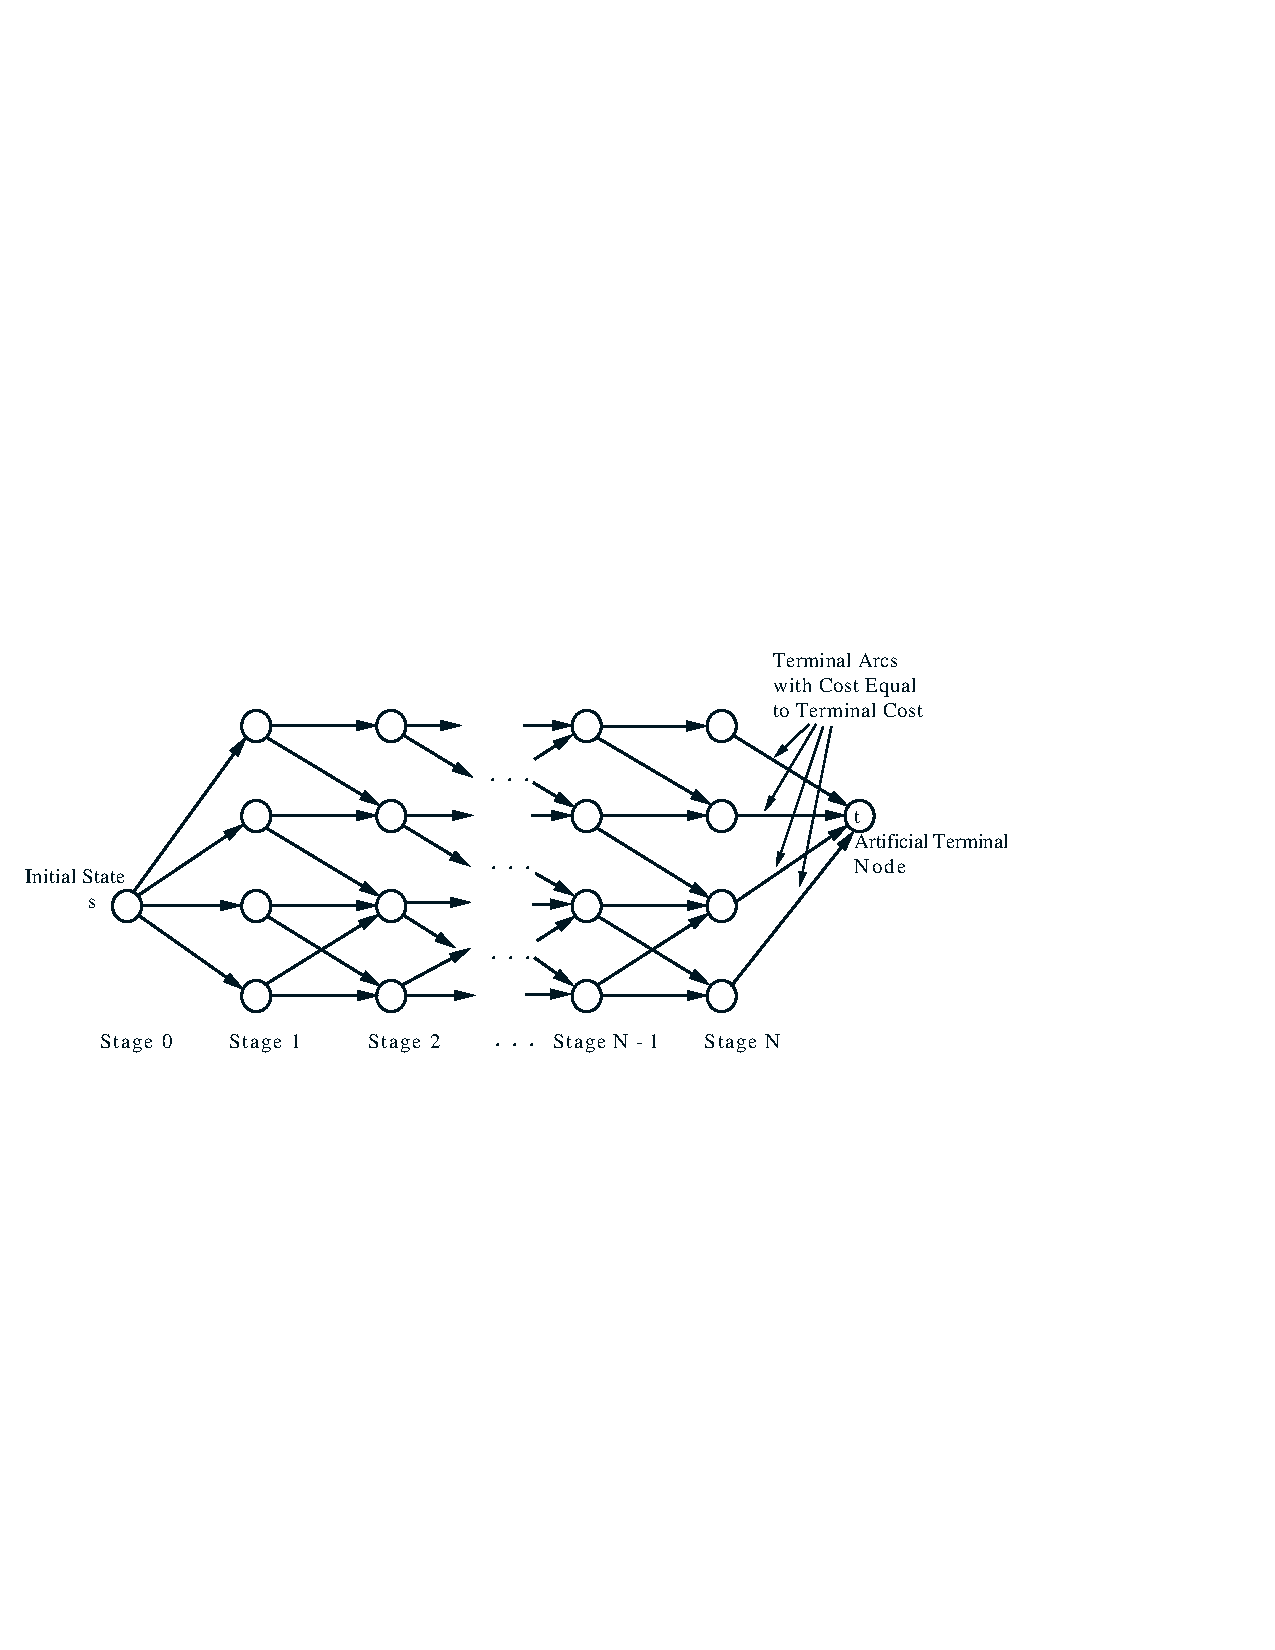
\includegraphics{dp211.pdf}}
\end{center}

Si on numérote les noeuds couche par couche, par ordre croissant de 
valeur de $k$, on obtient un \emph{réseau sans cycle et ordonné topologiquement}
(i.e., un arc $(i,j)$ ne peut exister que si $i<j$).
Dans le cas où il n'est pas nécessaire de mémoriser le numéro 
d'étape, on peut simplifier le réseau en agrégeant des noeuds.
Le réseau résultant peut ne plus être ordonné topologiquement.
Inversement, tout problème de recherche d'un plus court chemin dans
un réseau peut se formuler comme un problème de programmation dynamique déterministe (avec des coûts additifs entre étapes).

\section{Cas probabiliste}

Dans la programmation dynamique probabiliste, la décision optimale à l'étape $n$ dépend de la loi de probabilité de l'état à l'étape $n+1$.
Ainsi, nous passerons de l'étape $n$ à l'étape $n+1$, se retrouvant ainsi dans l'état $i$, avec une probabilité $p_i$.
Étant donné $S$ états à l'étape $n+1$, nous aurons $p_i \geq 0$ et
\[
\sum_{i=1}^S p_i = 1.
\]
La relation de récurrence dépend de cette loi de probabilité et de l'objectif à optimiser.

\begin{example}[Jeu de hasard]
Le jeu consiste à miser un nombre quelconque de jetons.
Si nous gagnons, nous remportons le nombre de jetons misés.
Si nous perdons, nous perdons le nombre de jetons misés.
Un statisticien croit pouvoir gagner chaque jeu avec une probabilité égale à 2/3.
Ses collègues parient avec lui qu'en misant au départ 3 jetons, il aura moins de 5 jetons après 3 parties.
Combien de jetons miser à chacune des 3 parties?

Le modèle peut se formuler comme suit:  l'étape $n$ correspond à la partie $n$, $n = 1,2,3$ ($N = 3$).
L'état $s_n$ est le nombre de jetons au début de la partie $n$, et la décision $x_n$ correspond au nombre de jetons à parier à la partie $n$.
Nous souhaitons maximiser la probabilité d'avoir au moins 5 jetons après 3 parties.
Soit $f_n(s_n,x_n)$ la probabilité de terminer avec au moins 5 jetons, étant donné que nous sommes dans l'état $s_n$ à l'étape $n$, que nous misons $x_n$ jetons et que nous effectuons des décisions optimales aux étapes $n+1,\ldots,N$.
Nous avons
\[
 f_n^*(s_n) = \max \lbrace f_n(s_n,x_n) \,|\, x_n = 0,1,\ldots,s_n \rbrace.
\]
étant donné que nous dans l'état $s_n$ à l'étape $n$ et que nous misons $x_n$ jetons, nous pouvons:
\begin{itemize}
\item
perdre et se retrouver dans l'état $s_n - x_n$ avec une probabilité 1/3;
\item
gagner et se retrouver à l'état $s_n + x_n$ avec une probabilité 2/3.
\end{itemize}
Nous avons la fonction de récurrence
\[
f_n(s_n,x_n) = \frac{1}{3}f_{n+1}^*(s_n-x_n) + \frac{2}{3}f_{n+1}^*(s_n+x_n).
\]
De plus,
\[
f_4^*(s_4) =
\begin{cases}
0 &\mbox{ si } s_4 < 5, \\
1 &\mbox{ si } s_4 \geq 5.
\end{cases}
\]
Calculons d abord $f_3^*(s_3)$ et $x_3^*$.
Nous avons le tableau
\begin{center}
\begin{tabular}{|c|c|c|c|c|c|c|c|}
\hline
$s_3$ & $x_3 = 0$ & $x_3 = 1$ & $x_3 = 2$ & $x_3 = 3$ & $x_3 = 4$ & $f_3^*(s_3)$ & $x_3^*$ \\
\hline
0 & 0 & - & - & - & - & 0 & 0 \\
\hline
1 & 0 & 0 & - & - & - & 0 & $\geq 0 $\\
\hline
2 & 0 & 0 & 0 & - & - & 0 & $\geq 0 $\\
\hline
3 & 0 & 0 & $\frac{2}{3}$ & $\frac{2}{3}$ & - & $\frac{2}{3}$ & $\geq 2$\\
\hline
4 & 0 & $\frac{2}{3}$ & $\frac{2}{3}$ & $\frac{2}{3}$ & $\frac{2}{3}$ & $\frac{2}{3}$ & $\geq 1$\\
\hline
$\geq 5$ & 1 & & & & & 1 & 0 \\
\hline
\end{tabular}
\end{center}

Voyons maintenant comment nous pouvons calculer les valeurs $f_2^*(s_2)$ et $x_2^*$, lorsque $s_2 = 3$.
Il est clair que nous devons avoir $x_2 \leq 3$. De plus,
\begin{align*}
f_2(3,0) &= \frac{1}{3}f_3^*(3) + \frac{2}{3}f_3^*(3) = \frac{2}{3}; \\
f_2(3,1) &= \frac{1}{3}f_3^*(2) + \frac{2}{3}f_3^*(4) = \frac{4}{9}; \\
f_2(3,2) &= \frac{1}{3}f_3^*(1) + \frac{2}{3}f_3^*(5) = \frac{2}{3}; \\
f_2(3,3) &= \frac{1}{3}f_3^*(0) + \frac{2}{3}f_3^*(6) = \frac{2}{3}. \\
\end{align*}
Ainsi,
\[
f_2^*(3) = \max \lbrace f_2(3,0), f_2(3,1), f_2(3,2), f_2(3,3) \rbrace = f_2(3,0).
\]
Dès lors, $x_2^* = 0$, $2$ ou $3$.
De la même façon, pour $s_2$, nous avons le tableau,
\begin{center}
\begin{tabular}{|c|c|c|c|c|c|c|c|}
\hline
$s_2$ & $x_2 = 0$ & $x_2 = 1$ & $x_2 = 2$ & $x_2 = 3$ & $x_2 = 4$ & $f_2^*(s_2)$ & $x_2^*$ \\
\hline
0 & 0 & - & - & - & - & 0 & 0 \\
\hline
1 & 0 & 0 & - & - & - & 0 & $\geq 0 $\\
\hline
2 & 0 & $\frac{4}{9}$ &  $\frac{4}{9}$ & - & - &  $\frac{4}{9}$ & $1,2$\\
\hline
3 & $\frac{2}{3}$ & $\frac{4}{9}$ & $\frac{2}{3}$ & $\frac{2}{3}$ & - & $\frac{2}{3}$ & $0,2,3$\\
\hline
4 & $\frac{2}{3}$ & $\frac{8}{9}$ & $\frac{2}{3}$ & $\frac{2}{3}$ & $\frac{2}{3}$ & $\frac{8}{9}$ & $\geq 1$\\
\hline
$\geq 5$ & 1 & & & & & 1 & 0 \\
\hline
\end{tabular}
\end{center}
Pour la première étape ($n = 1$), nous avons $s_1 = 3$, comme nous pouvons affecter 3 jetons au départ du jeu.
Ceci donne le tableau
\begin{center}
\begin{tabular}{|c|c|c|c|c|c|c|}
\hline
$s_1$ & $x_1 = 0$ & $x_1 = 1$ & $x_1 = 2$ & $x_1 = 3$ & $f_1^*(s_2)$ & $x_1^*$ \\
\hline
3 & $\frac{2}{3}$ & $\frac{20}{27}$ & $\frac{2}{3}$ & $\frac{2}{3}$ & $\frac{20}{27}$ & 1 \\
\hline
\end{tabular}
\end{center}
Dès lors
\begin{align*}
 f_1(3,0) &= \frac{1}{3}f_2^*(3) + \frac{2}{3}f_2^*(3) = \frac{2}{3}, \\
 f_1(3,1) &= \frac{1}{3}f_2^*(2) + \frac{2}{3}f_2^*(4) = \frac{20}{27}, \\
 f_1(3,2) &= \frac{1}{3}f_2^*(1) + \frac{2}{3}f_2^*(5) = \frac{2}{3}, \\
 f_1(3,3) &= \frac{1}{3}f_2^*(0) + \frac{2}{3}f_2^*(6) = \frac{2}{3},
 \end{align*}
 et par conséquent,
 \[
 f_1^*(3) = \max \lbrace f_1(3,0), f_1(3,1), f_1(3,2), f_1(3,3) \rbrace = f_1(3,1).
 \]
 Nous en déduisons
 \[
 x_1^* = 1.
 \]
La politique optimale est donc :
\begin{itemize}
\item
$x_1^* = 1$;
\item
Si nous gagnons ($s_2 = 4$), $x_2^* = 1$.
\begin{itemize}
\item
Si nous gagnons ($s_3 = 5$), $x_3^* = 0$.
\item
Si nous perdons ($s_3 = 3$), $x_3^* = 2$ ou $3$.
\end{itemize}
\item
Si nous perdons ($s_2 = 2$), $x_2^* = 1$ ou $2$.
\begin{itemize}
\item
Si nous gagnons ($s_3 = 3$ ou $4$), $x_3^* = 2$ ou $3$ (si $x_2^* = 1$) ou
$1 \leq x_3^* \leq 4$ (si $x_2^* = 2$).
\item
Si nous perdons ($s_3 = 1$ ou $0$), $x_3^* \geq 0$ (mais le pari est perdu!).
\end{itemize}
\end{itemize}
\end{example}

\begin{small}
\section{Notes}

Ce chapitre se base essentiellement sur les notes de cours de Bernard Gendron, 2007. Le lien avec les plus courts chemins est tiré du cours IFT6521 donné au département d'informatique et de recherche opérationnelle de l'Université de Montréal (Pierre L'Ecuyer, Fabian Bastin).

\end{small}
